\documentclass{article}
\usepackage{times}
\usepackage{balance}
\usepackage{amssymb}
\usepackage{amsfonts}
\usepackage{amsmath}
\usepackage[amsmath,thmmarks]{ntheorem}
\usepackage{mathrsfs}
\usepackage[utf8]{inputenc}
\usepackage{listings}              % code insert
\usepackage{graphicx}

\newcommand{\R}{\mathbb{R}}
\newcommand{\C}{\mathbb{C}}
\newcommand{\Z}{\mathbb{Z}}
\newcommand{\id}{\textrm{id}}
\newcommand{\pr}{\mathrm{pr}}
\newcommand{\N}{\mathbb{N}}


\newtheorem{thm}[equation]{Theorem}
\newtheorem{lem}[equation]{Lemma}
\newtheorem{prop}[equation]{Proposition}
\newtheorem{cor}[equation]{Corollary}
\newtheorem{conj}[equation]{Conjecture}

\theoremstyle{plain}
\theorembodyfont{\normalfont}
\newtheorem{defn}[equation]{Definition}
\newtheorem{ex}[equation]{Example}
\newtheorem{claim}[equation]{Claim}

\theoremstyle{nonumberplain}
\theoremheaderfont{\normalfont\bfseries}
\theorembodyfont{\normalfont}
\theoremsymbol{\ensuremath{\square}}
\theoremseparator{.}
\newtheorem{proof}{Proof}


\pagestyle{plain}

\begin{document}

\title{Advanced Computer Systems \\ Assignment 2}

\author{Anna Sofie Kiehn and Kenneth Jürgensen}

\maketitle

\section{Serializability and Locking}

\subsection{Precedence graph}

The precedence graphs for schedule 1 and schedule 2 can be seen in Figure 1. 

\begin{figure}[h]
    \centering
    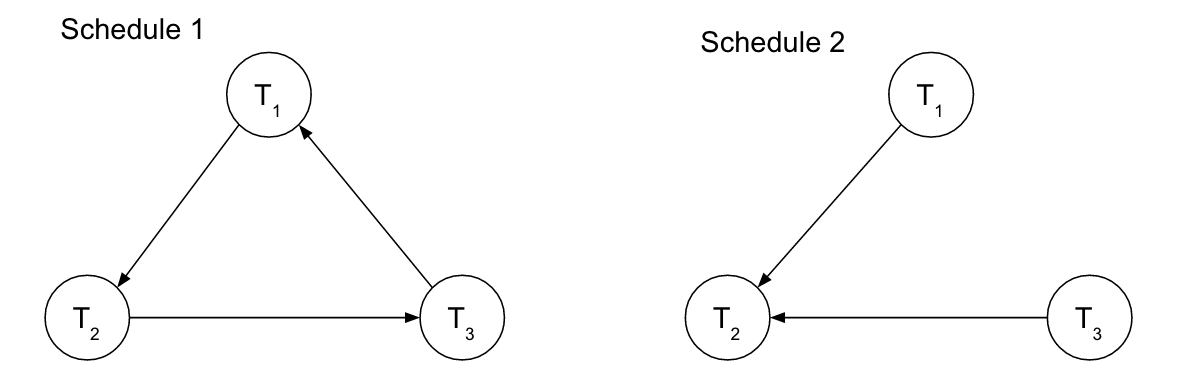
\includegraphics[width=14cm]{graph}
    \caption{Precedence graph for schedule 1 and schedule 2}
\end{figure} 

As can be seen in the graphs, schedule 1 cannot be syncronized as there is a cycle in the graph. Schedule 2 can be syncronized as it contains no cycle. 

\subsection{Can the schedules be generated using strict 2PL}

\section{Optimistic Concurrency Control}

\subsection{Scenario 1}

\subsection{Scenario 2}

\subsection{Scenario 3}

\section{Programming task}


\end{document}